\documentclass[bachelor, och, otchet]{template}

\usepackage[utf8]{inputenc}
\usepackage{graphicx}

\usepackage{pdfpages}
\usepackage{amsmath}

\usepackage[sort,compress]{cite}
\usepackage{amsmath}
\usepackage{amssymb}
\usepackage{amsthm}
\usepackage{fancyvrb}
\usepackage{longtable}
\usepackage{array}
\usepackage[english,russian]{babel}
\usepackage{minted}

\usepackage{tempora}

\usepackage[justification=centering]{caption}
\usepackage[colorlinks=false, hidelinks=true]{hyperref}


\newcommand{\eqdef}{\stackrel {\rm def}{=}}


\begin{document}

\title{Практические задания по курсу <<Нейронные сети>>}

\course{5}

\group{531}

\napravlenie{10.05.01 "--- Компьютерная безопасность}


\author{Токарева Никиты Сергеевича}


\satitle{доцент}
\saname{И.\,И.\, Слеповичев}


\date{2023}

\maketitle

% Включение нумерации рисунков, формул и таблиц по разделам
% (по умолчанию - нумерация сквозная)
% (допускается оба вида нумерации)
%\secNumbering


% \tableofcontents

\section{Создание ориентированного графа}

\subsection{Описание задачи №1}
\textbf{На вход:} текстовый файл с описанием графа в виде списка дуг:

\begin{center}
    $(a_1, b_1, n_1), (a_2, b_2, n_2), \dots (a_k, b_k, n_k)$,
\end{center}

где $a_i$ -- начальная вершина дуги $i$, $b_i$ -- конечная вершина дуги $i$ ($a_i \neq b_i$), $n_i$ -- порядковый номер дуги
в списке всех заходящих в вершину $b_i$ дуг. Т.е. допустим в ориентированном графе будут заданы дуги, например $(a_1, b_1)$ и $(a_2, b_1)$,
тогда в описании данного графа будут заданы дуги $(a_1, b_1, n_1)$ и $(a_2, b_1, n_2)$, где номера этих дуг упорядоченны и различны.

\textbf{На выходе:}

\begin{itemize}
    \item[а)] Ориентированный граф с именованными вершинами и линейно упорядоченными дугами (в соответствии с порядком из текстового файла).
    Структура графа должна записываться в файл формата XML или JSON.
    \item[б)] Сообщение об ошибке в формате файла, если ошибка присутствует.
\end{itemize}

\subsection{Примеры исполнения программы}

\textbf{Пример №1}:

Рассмотрим ориентированный граф, который имеет следующую запись:

\begin{center}
    $(v1, v2, 1),(v3, v4, 1),(v2, v5, 1),(v5, v6, 1),(v5, v7, 1),$ \\ $(v4, v8, 1),(v4, v9, 1), (v9, v6, 2)$
\end{center}

Этот граф можно представить в следующем виде, как показано на рисунке \ref{p1}.

\begin{figure}[H]
    \centering
    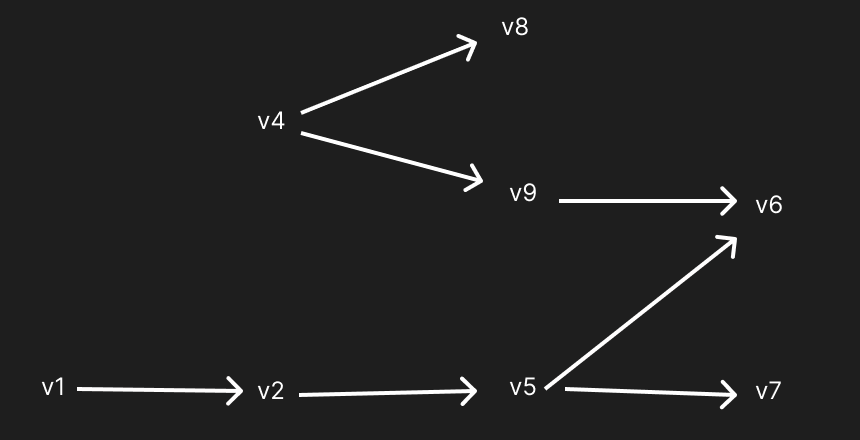
\includegraphics[width=0.7\textwidth]{pics/1.1.png}
    \caption{Изображение ориентированного графа}
    \label{p1}
\end{figure} 

Тогда после выполнении программы результатом будет являться следующая структура, которая
будет записана в файл формата JSON.

\begin{minted}{JSON}
    {
        "graph": 
        {
            "vertex": 
            [
                "v1", "v2", "v3", "v4", "v5", 
                "v6", "v7", "v8", "v9"
            ], 
            "arc": 
            [
                {"from": "v1", "to": "v2", "order": 1}, 
                {"from": "v3", "to": "v4", "order": 1}, 
                {"from": "v2", "to": "v5", "order": 1}, 
                {"from": "v5", "to": "v6", "order": 1}, 
                {"from": "v5", "to": "v7", "order": 1}, 
                {"from": "v4", "to": "v8", "order": 1}, 
                {"from": "v4", "to": "v9", "order": 1}, 
                {"from": "v9", "to": "v6", "order": 2}
            ]
        }
    }
    \end{minted}

\textbf{Пример 2:}

Рассмотрим ориентированный граф, который имеет следующую запись:

\begin{center}
    $(a, b, 1),(c, d, 1),(b, e, 1),(d, e, 1),(e, f, 1)$
\end{center}

На рисунке \ref{p2} показано изображение данного графа.

\begin{figure}[H]
    \centering
    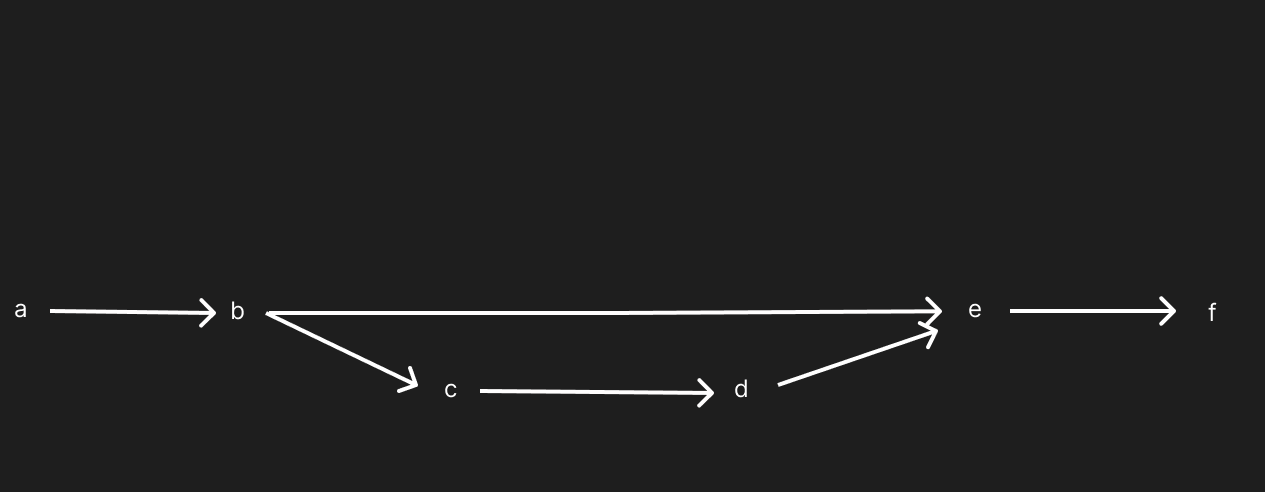
\includegraphics[width=0.7\textwidth]{pics/1.2.png}
    \caption{Изображение ориентированного графа}
    \label{p2}
\end{figure} 

Исходя из рисунка, можно заметить, что такой вариант графа вполне допустим, однако в описании дуг
была допущена ошибка: дуги $(b, e, 1)$ и $(d, e, 1)$ имеют одинаковый порядковый 
номер. В таком случае программа выводит сообщение об ошибке, что в графе некорректно заданы
номера.

\section{Создание функции по графу}

    \subsection{Описание задачи №2}

        \textbf{На входе:} ориентированный граф с именованными вершинами как 
        описано в задании 1.
        
        \textbf{На выходе:} линейное представление функции, реализуемой графом в префиксной скобочной записи:

            \begin{center}
                $A_1(B_1(C_1(\dots), \dots, C_m(\dots)), \dots, B_n(\dots))$
            \end{center}

        \textbf{Способ проверки резульата:}
            \begin{itemize}
                \item[а)] выгрузка в текстовый файл результата преобразования графа в имя функции.
                \item[б)] сообщение о наличии циклов в графе, если они присутствуют.
            \end{itemize}
        
    \subsection{Примеры исполнения программы}


    \textbf{Пример 1:}

    Рассмотрим ориентированный граф, который имеет следующую запись:

    \begin{center}
        $(v1, v2, 1), (v3 , v2, 2), (v2, v4, 1), (v4, v5, 1)$
    \end{center}

    На рисунке \ref{p21} показано изображение данного графа.

    \begin{figure}[H]
        \centering
        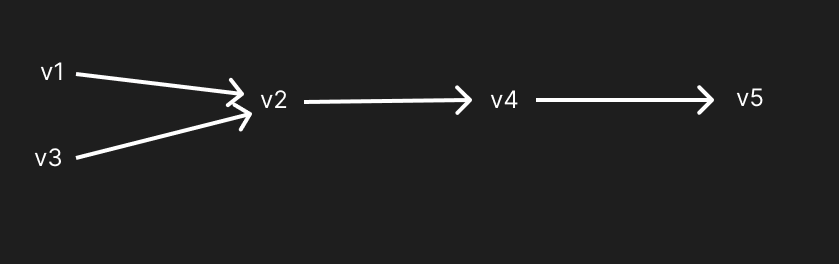
\includegraphics[width=0.7\textwidth]{pics/2.1.png}
        \caption{Изображение ориентированного графа}
        \label{p21}
    \end{figure} 

    В результате работы программы в файл будет сделана следующая запись:

    \begin{center}
        $v5(v4(v2(v1(), v3())))$
    \end{center}


    \textbf{Пример 2:}

    Рассмотрим ориентированный граф, который имеет следующую запись:

    \begin{center}
        $(v1, v2, 1), (v2, v3, 1), (v3, v1, 1)$
    \end{center}

    На рисунке \ref{p22} показано изображение данного графа.

    \begin{figure}[H]
        \centering
        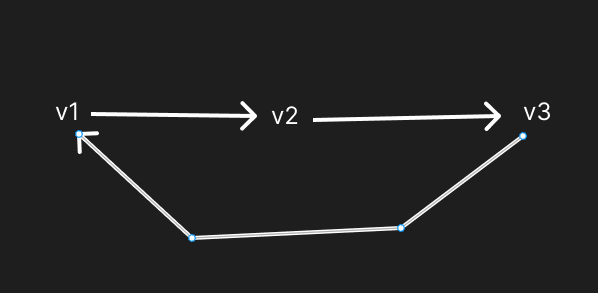
\includegraphics[width=0.7\textwidth]{pics/2.2.png}
        \caption{Изображение ориентированного графа}
        \label{p22}
    \end{figure} 

    Исходя из рисунка, видно, что в данном графе присутствует цикл. Поэтому результатом
    программы будет вывод об ошибке в консоль.


\section{Вычисление значение функции на графе}

    \subsection{Описание задачи №3}

    \textbf{На входе:} 

        \begin{itemize}
            \item[а)] Текстовый файл с описанием графа в виде списка дуг (смотри задание 1).
            \item[б)] Текстовый файл соответствий арифметических операций именам вершин:
            
                \begin{center}
                    $a_1 : 1\text{-я операция}$ \\
                    $a_2 : 2\text{-я операция}$ \\
                    $\dots$ \\
                    $a_n : n\text{-я операция}$, \\
                \end{center}
                где $a_i$ -- имя $i$-й вершины, $i$-я операция -- символ операции, соответствующий вершине $a_i$.
                
                Допустимы следующие символы операций: \\
                $+$ -- cумма значений,\\
                $*$ -- произведение значений,\\
                $exp$ -- экспонирование входного значения,\\
                число -- любая числовая константа.\\		
        \end{itemize}

    \textbf{На выходе:} значение функции, построенной по графу а) и файлу б).

    \textbf{Способ проверки результата:} результат вычисления, выведенный в файл.

    \subsection{Примеры исполнения программы}
    
    \textbf{Пример 1:}

    Рассмотрим ориентированный граф, который имеет следующую запись:

    \begin{center}
        $(v1, v2, 1), (v1, v2, 2), (v2, v6, 1), (v3, v5, 1), (v4, v5, 2), (v6, v7, 1), (v5, v7, 2)$
    \end{center}

    Также имеются соответствия арифметических операций именам вершинам, записанных в файле формата JSON:

    \begin{minted}{JSON}
        {
            "v1" : 1,
            "v2" : "+",
            "v3" : 5,
            "v4" : 12,
            "v5" : "*",
            "v6" : "exp",
            "v7" : "+"
        }
    \end{minted}
    
    На рисунке \ref{p31} показано изображение данного графа.

    \begin{figure}[H]
        \centering
        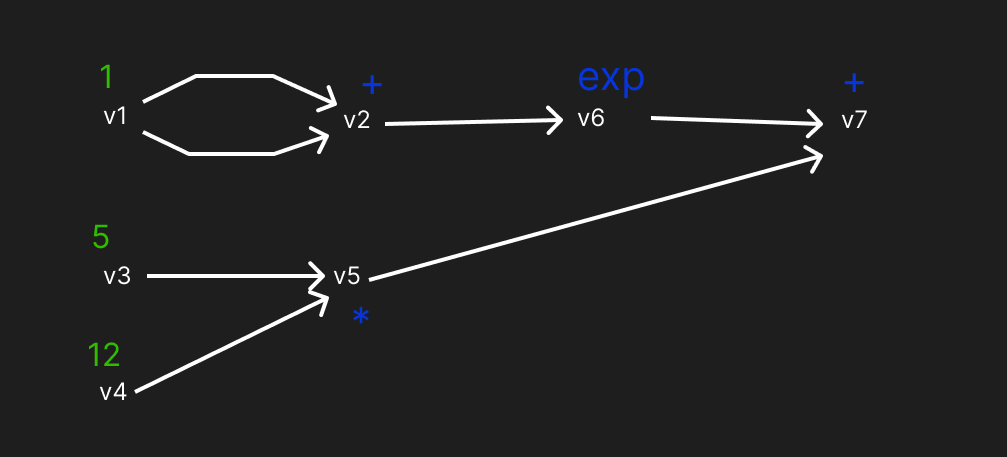
\includegraphics[width=0.7\textwidth]{pics/3.1.png}
        \caption{Изображение ориентированного графа}
        \label{p31}
    \end{figure} 

    После всех проверок входных данных на корректность, программа 
    представляет ориентированный граф в следующем виде:
    
    \begin{center}
        $v7(v6(v2(v1(), v1())), v5(v3(), v4()))$
    \end{center}

    Подставив в соответствие именам вершин арифметические операции получается следующая запись:

    \begin{center}
        $+(exp(+(1, 1)), *(5, 12))$
    \end{center}

    Таким образом программе необходимо вычислить выражение, представленное в префиксной записи.
    В итоге программа записывает в текстовый файл результат данного выражения: 67.38905609893065.

    \textbf{Пример 2:}

    Теперь рассмотрим ориентированный граф, который имеет достаточную простую запись:

    \begin{center}
        $(v1, v3, 1), (v2, v3, 2)$
    \end{center}

    Также имеются следующие соответствия:

    \begin{minted}{JSON}
        {
            "v1" : 1,
            "v2" : "+",
            "v3" : 5
        }
    \end{minted}
    
    На рисунке \ref{p32} показано изображение данного графа.

    \begin{figure}[H]
        \centering
        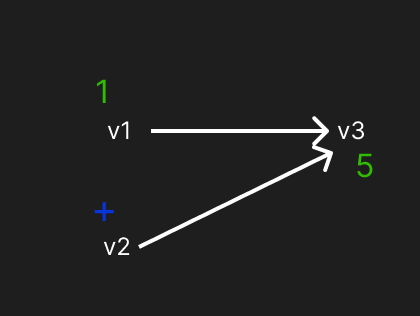
\includegraphics[width=0.7\textwidth]{pics/3.2.png}
        \caption{Изображение ориентированного графа}
        \label{p32}
    \end{figure} 

    Исходя из рисунка и текущих соответствий, можно заметить, что в данном случае невозможно
    будет вычислить результат. Поэтому программа выдает в качестве ответа в консоль сообщение
    об ошибке.

\section{Построение многослойной нейронной сети}

\subsection{Описание задачи №4}

    \textbf{На входе:} 

    \begin{itemize}
        \item[а)] Файл с набором матриц весов межнейронных связей:
        \begin{center}
            $M_1 : [a_{11}^1, a_{12}^1, \dots, a_{1n_1}^1], \dots, [a_{m_11}^1, a_{m_12}^1, \dots ,a_{m_1n_1}^1]$ \\
            $M_2 : [a_{11}^2, a_{12}^2, \dots, a_{1n_2}^2], \dots, [a_{m_21}^2, a_{m_22}^2, \dots ,a_{m_2n_2}^2]$\\
            $\dots$\\
            $M_p : [a_{11}^p, a_{12}^p, \dots, a_{1n_p}^p], \dots, [a_{m_p1}^p, a_{m_p2}^p, \dots,a_{m_pn_p}^p]$ \\                  
        \end{center}
        \item[б)] Файл с входным вектором в формате:
        
        \begin{center}
            $x_1, x_2, \dots, x_k$.
        \end{center}
    \end{itemize}

    \textbf{На выходе:}
        \begin{itemize}
            \item[а)] Сериализованная многослойная нейронная сеть (в формате XML или JSON) с полносвязной межслойной структурой. 
            Файл с выходным вектором -- результатом вычислений НС в формате: 
            \begin{center}
                $y_1, y_2, \dots, y_k.$                
            \end{center}
            \item[б)] Сообщение об ошибке, если в формате входного вектора или файла описания НС допущена 
            ошибка.
        \end{itemize}
        

\subsection{Примеры исполнения программы}

        \textbf{Пример 1:}

        Пусть заданы следующие матрицы весов $M_1 = [[1], [2], [3]]$ размерности (3 x 1)
        и $M_2 = [[4, 5, 6]]$ размерности (1 х 3), записанные в файл формата JSON:
        
        \begin{minted}{JSON}
            {
                "W" : 
                [
                    [
                        [1], [2], [3]
                    ], 
                    [
                        [4, 5, 6]
                    ]
                ]
            }
        \end{minted}

        Также в качестве входного вектора выступают значения $x = [[0.1], [0.2], [0.3],$ \\$[0.4], [0.5]]$, 
        которые записаны в файл формата JSON.

        \begin{minted}{JSON}
            {
                "x" : [[0.1], [0.2], [0.3], [0.4], [0.5]]
            }
        \end{minted}

        В данной задаче, чтобы получить выходной вектор необходимо выполнять умножение каждого элемента входного вектора на
        матрицу весов $M_i$, после каждого такого умножения также нужно поэлементно применить функцию активации. В программе функцией
        активации по умолчанию является сигмоидальная функция:
        
        \begin{center}
            $f(x) = \frac{1}{1 + e^{-x}}$.
        \end{center}

        Так как в данном случае $|x| = 5$, то относительно каждого элемента вектора $x = [x_1, x_2, x_3, x_4, x_5]$ 
        выполняются следующие действия:

        \begin{enumerate}
            \item Умножение матрицы весов $M_1$ на вектор $x_i$ $(1 \leq i \leq 5)$: $out_1 = M_1 \cdot x_i$.
            Если умножение выполнить не удалось из-за того что два множителя несовместимы, то в консоль программа
            выводит сообщение об ошибке;
            \item Поэлементое применение функции $f(x)$ к $out_1$, в результате чего получается выходной вектор $y_1^{i}$;
            \item Для $k = 2 \dots p$, где $p$ -- количество матриц весов, выполнять шаги 4-6.
            \item Умножение матрицы весов $M_k$ на вектор $y_{k - 1}^{i}$ $(1 \leq i \leq 5)$: $out_k = M_k \cdot x_i$.
            Если умножение выполнить не удалось из-за того что два множителя несовместимы, то в консоль программа
            выводит сообщение об ошибке;
            \item Поэлементое применение функции $f(x)$ к $out_k$, в результате чего получается выходной вектор $y_k^{i}$;
            \item Если $k = p$, то в качестве результата вернуть выходной вектор $y_k^{i}$, иначе увеличить $k$ на единицу.
        \end{enumerate}

        Стоит отметить, что для корректной работы программы во входных данных очень важно следить за тем, чтобы при умножении
        матрицы были совместимыми (число столбцов первого множителя равно числу строк второго множителя).
        
        Так как в данном случае все условия для корректной работы программы выполняются, то получается следующий выходной вектор:

        \begin{minted}{JSON}
            {
                "y": 
                [
                    [0.9997504849648627], [0.9998845678407059], 
                    [0.9999440920809696], [0.999971219155923], 
                    [0.9999841222683092]
                ]
            }
            
        \end{minted}

        \textbf{Пример 2:}

        Пусть заданы следующие матрицы весов $M_1 = [[1], [2], [3]]$ размерности (3 x 1)
        и $M_2 = [[4, 5, 6, 7]]$ размерности (1 х 4), записанные в файл формата JSON:
        
        \begin{minted}{JSON}
            {
                "W" : 
                [
                    [
                        [1], [2], [3]
                    ], 
                    [
                        [4, 5, 6, 7]
                    ]
                ]
            }
        \end{minted}

        Также в качестве входного вектора выступают значения $x = [[0.1], [0.2], [0.3],$ \\$[0.4], [0.5]]$, 
        которые записаны в файл формата JSON.

        \begin{minted}{JSON}
            {
                "x" : [[0.1], [0.2], [0.3], [0.4], [0.5]]
            }
        \end{minted}

        В данном случае программа выдает ошибку во время попытки умножения матрицы $M_2$ на результирующую матрицу,
        полученную после умножения матрицы $M_1$ и применения функции активации $f(x)$. При умножении $x_i$ на матрицу $M_1$,
        у результирующего вектора число строк стало равно числу строк матрицы $M_1$. Так как в данном случае у матрицы $M_2$ число
        столбцов не совпадает с числом строк результирующего вектора, то дальнейшее выполнение программы невозможно, и она выводит 
        в консоль сообщение об ошибке.

        
    
\section{Реализация метода обратного распространения ошибки для многослойной НС}

    \subsection{Описание задачи №5}

        \textbf{На входе:}
        
            \begin{itemize}
                \item[а)] Текстовый файл с описанием НС (формат см. в задании 4).
                \item[б)] Текстовый файл с обучающей выборкой:
                
                    \begin{center}
                        $[x_{1}^{1}, x_{2}^1, \dots, x_{k}^1] \rightarrow [y_{1}^1, y_{2}^1, \dots, y_{l}^1]$ \\
                        $\dots$\\
                        $[x_{1}^n, x_{2}^n, \dots, x_{k}^n] \rightarrow [y_{1}^n, y_{2}^n, \dots, y_{l}^n]$ \\
                    \end{center}
                    Формат описания входного вектора $x$ и выходного вектора $y$ соответствует формату из задания 4. 
                \item[в)] Число итераций обучения (в строке параметров).

            \end{itemize}

        \textbf{На выходе:} Текстовый файл с историей $N$ итераций обучения методом обратного распространения ошибки:
            \begin{center}
                $1 : \text{1-я ошибка}$ \\
                $2 : \text{2-я ошибка}$ \\
                    $\dots$\\
                $N : \text{N-я ошибка}$ \\

            \end{center}

    \subsection{Примеры исполнения программы}

    \textbf{Пример:}

        Пусть заданы следующие матрицы весов $M_1 = [[1], [2], [3]]$ размерности (3 x 1)
        и $M_2 = [[4, 5, 6]]$ размерности (1 х 3), записанные в файл формата JSON:
        
        \begin{minted}{JSON}
            {
                "W" : 
                [
                    [
                        [1], [2], [3]
                    ], 
                    [
                        [4, 5, 6]
                    ]
                ]
            }
        \end{minted}
    
        В другом JSON-файле записана обучающая выборка в следующем виде:
        
        \begin{minted}{JSON}
            { 
                "in" : 
                [
                    [0.1], [0.2], [0.3], [0.4]
                ], 
                "out" : 
                [
                    [0.9], [0.8], [0.7], [0.6]
                ] 
            }
        \end{minted}

        Обозначим обучающую выборку входных параметров как вектор $x$, а выборку выходных параметров -- $d$.
        Также в отдельном файле записаны дополнительные параметры: количество итераций $m = 25$ и коэффициент
        скорости обучения ($0 < lrate < 1$)  $lrate = 0.6$.

        Обратное распространение ошибки состоит из следующих шагов:

        \begin{enumerate}
            \item Для $r = 1, \dots m$ выполнять шаги 2 - 6.
            \item Прямое распространение сигнала. Входные сигналы передаются по сети от 
            нейрона к нейрону. Каждый нейрон вычисляет свою активационную функцию от входных 
            данных и передает результат следующему нейрону. При выполнении данного шага применяется алгоритм,
            реализованный в задаче №4. Однако стоит отметить, что дополнительно запоминаются промежуточные 
            выходные векторы $y_j^i$ ($0 \leq j \leq p$, $1 \leq i \leq k$, $p$ -- количество слоев (матриц весов), $k$ -- количество элементов
            в векторе $x$), полученные после каждого слоя. Стоит отметить, что вектор $y_0^i = x_i^{s}$ ($1 \leq s \leq n$), т.е. после
            выполнения прямого распространения сигнала должна получится последовательность векторов $y_0^i = x_i^{s}, y_1^i, \dots y_p^i$.
            \item Вычисление ошибки. После прямого распространения сигнала 
            вычисляется разница между полученными и ожидаемыми выходными значениями сети. 
            Эта разница является ошибкой, которую необходимо минимизировать. В программной реализации $i$-я
            ошибка $e$ вычисляется, как $e = y_p^i - d_i$.  
            \item Обратное распространение ошибки. Ошибка сети распространяется в обратном направлении, от выходных нейронов к входным. 
            Каждый нейрон вычисляет градиент ошибки по отношению к его входным данным и весам связей. Градиент ошибки $grad$ относительно
            последнего слоя вычисляется по формуле $grad_p = e \cdot f^{'}(y_p^i)$.
            \item Обновление весов. Используя градиент ошибки, веса связей между нейронами корректируются с помощью заданного 
            обновления весового коэффициента. Целью является минимизация ошибки и улучшение результатов сети. Обновление весов происходит 
            следующем образом:

            \begin{enumerate}
                \item Обновление весов последнего $p$-го слоя $M_p$: \\$M_p = M_p - lrate \cdot y_{p - 1}^i \cdot grad_p$;
                \item Для $t = p - 1 \dots 1$ выполнять следующее: вычислить \\$grad_t = M_{t + 1} \cdot grad_{t + 1} \cdot f^{'}(y_{t}^i)$,
                затем выполнить обновление весов матрицы $M_t$: $M_t = M_t - y_{t-1}^i \cdot grad_t \cdot lrate$. Причем размерность матриц весов
                должна сохраняться, чтобы корректно посчитать последующие значения обучающей выборки.
            \end{enumerate}
            \item Далее после прохождения по всем значениям $x_i^s$. ($1 \leq i \leq k$, $1 \leq s \leq n$) вычисляется среднее арифметическое значений
            ошибки $\mu = \frac{e_1 + \dots + e_k}{k}$ и сохраняется в отдельный список. После чего количество итераций увеличивается на единицу. 
        \end{enumerate}

        Таким образом результатом работы программы является сообщение следующего вида, которое записывается в текстовый файл:

        \begin{center}
            При i = 1 значения функции ошибок: 0.24965137935543213\\
            При i = 2 значения функции ошибок: 0.24944708478343486\\
            При i = 3 значения функции ошибок: 0.2494469476387328\\
            При i = 4 значения функции ошибок: 0.24944681042609376\\
            При i = 5 значения функции ошибок: 0.24944667314546723\\
            При i = 6 значения функции ошибок: 0.2494465357968028\\
            При i = 7 значения функции ошибок: 0.24944639838004992\\
            При i = 8 значения функции ошибок: 0.24944626089515787\\
            При i = 9 значения функции ошибок: 0.24944612334207614\\
            При i = 10 значения функции ошибок: 0.24944598572075405\\
            При i = 11 значения функции ошибок: 0.24944584803114084\\
            При i = 12 значения функции ошибок: 0.2494457102731858\\
            При i = 13 значения функции ошибок: 0.24944557244683785\\
            При i = 14 значения функции ошибок: 0.24944543455204632\\
            При i = 15 значения функции ошибок: 0.24944529658876027\\
            При i = 16 значения функции ошибок: 0.24944515855692864\\
            При i = 17 значения функции ошибок: 0.24944502045650035\\
            При i = 18 значения функции ошибок: 0.2494448822874244\\
            При i = 19 значения функции ошибок: 0.2494447440496496\\
            При i = 20 значения функции ошибок: 0.24944460574312483\\
            При i = 21 значения функции ошибок: 0.24944446736779877\\
            При i = 22 значения функции ошибок: 0.2494443289236201\\
            При i = 23 значения функции ошибок: 0.24944419041053753\\
            При i = 24 значения функции ошибок: 0.24944405182849969\\
            При i = 25 значения функции ошибок: 0.24944391317745518 \\  
        \end{center}

\end{document}